\section{Preliminary Methods}
\begin{figure}[t!]
	\centering
	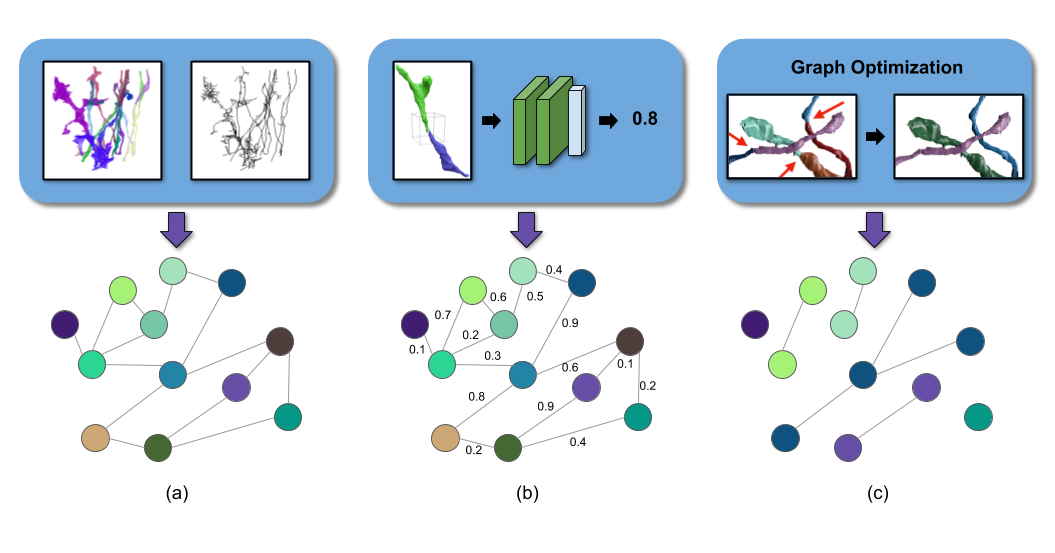
\includegraphics[width=\linewidth]{./figures/teaser_v4.png}
	\caption{Our framework uses both geometric and topological biological constraints for region merging. We (a) generate a simplified graph from the skeleton representation of the input segmentation, (b) train a classifier to learn the edge weight based on the shape of the segment connection, and (c) perform graph partitioning with acyclic constraints.}
	\label{fig:teaser_pipeline}
\end{figure}

\paragraph{Biologically-Constrained Error Correction}

Our method is illustrated in Fig.~\ref{fig:teaser_pipeline}.
From the input segmentation we generate a graph $G$ with nodes $N$ and edges $E$ with weights $w_e$. 
The nodes correspond to labeled segments from the input data with edges between merge candidates.
We propose the following three steps to formulate and then partition the graph while obeying constraints from the underlying biology.
First, we only consider merging segments based on a skeletonized representation of the input segmentation (Fig.~\ref{fig:teaser_pipeline}a).
This enables us to reduce the number of nodes in the graph based on prior knowledge on the shape of neuronal processes.
Second, we train a convolutional neural network that learns biological constraints based on the shapes of the input segmentation (Fig.~\ref{fig:teaser_pipeline}b).
This network generates probabilities that segments belong to the same neuron based only on the segmentations. 
An example of one such learned constraint is that neurons have small turning radii (Fig.~\ref{fig:turn-radii}).
Third, we partition the graph using a lifted multicut formulation with additional acyclic constraints to enforce global biological constraints (Fig.~\ref{fig:teaser_pipeline}c).
The lifted multicut solution is globally consistent which we then augment to produce a tree-structured graph (i.e., one with no cycles).

\subsection{Skeleton-Based Graph Generation}
%\subsubsection{Node Generation}
\label{sec:skeletonization}
Most region merging methods create a region graph by removing small-sized segments and linking each pair of adjacent segments, which can still lead to a large graph size due to the irregular shape of neural structures.
We use a skeleton representation of the segmentation to reduce the graph size with the geometric constraints on the connectivity of two adjacent segments to prune edges.

\begin{figure}[t]
	\centering
	\begin{minipage}{0.45\linewidth}
		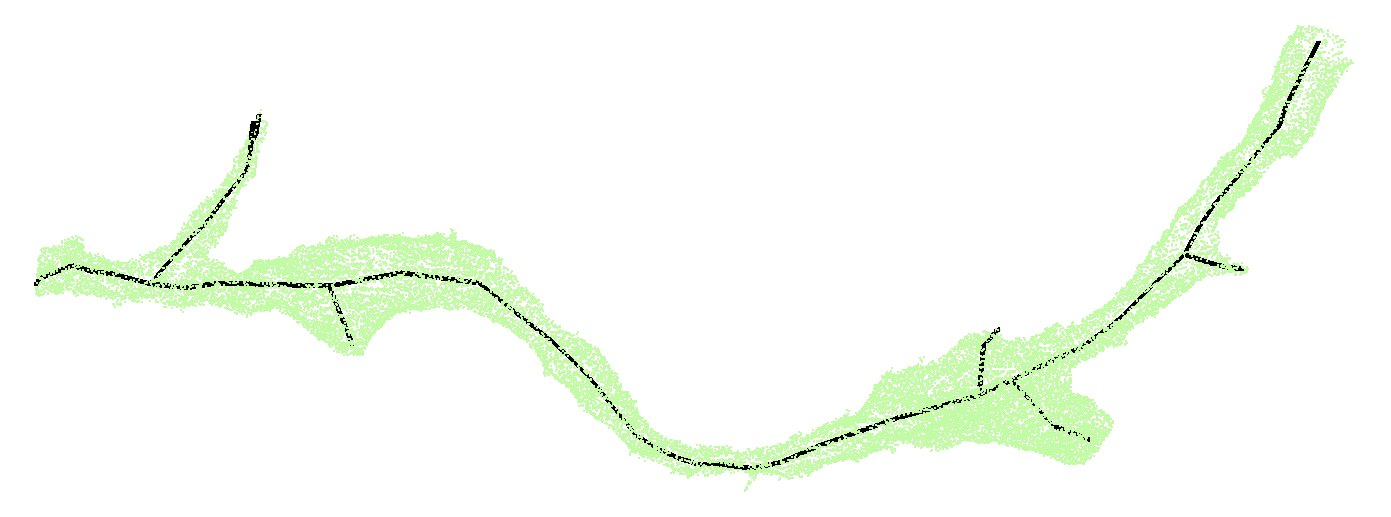
\includegraphics[width=\linewidth]{./figures/skeleton1.png}		
	\end{minipage}
	\hfill
	\begin{minipage}{0.45\linewidth}
		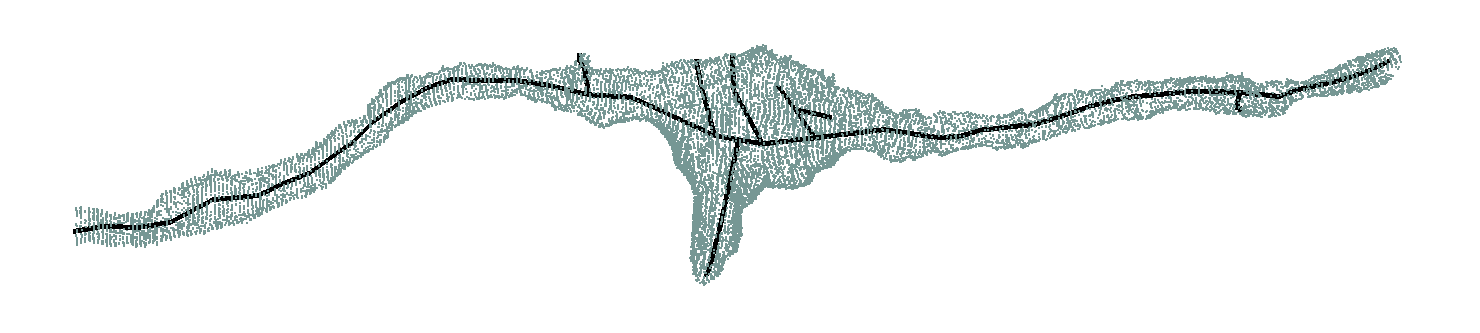
\includegraphics[width=\linewidth]{./figures/skeleton2.png}		
	\end{minipage}
	\begin{minipage}{0.45\linewidth}
		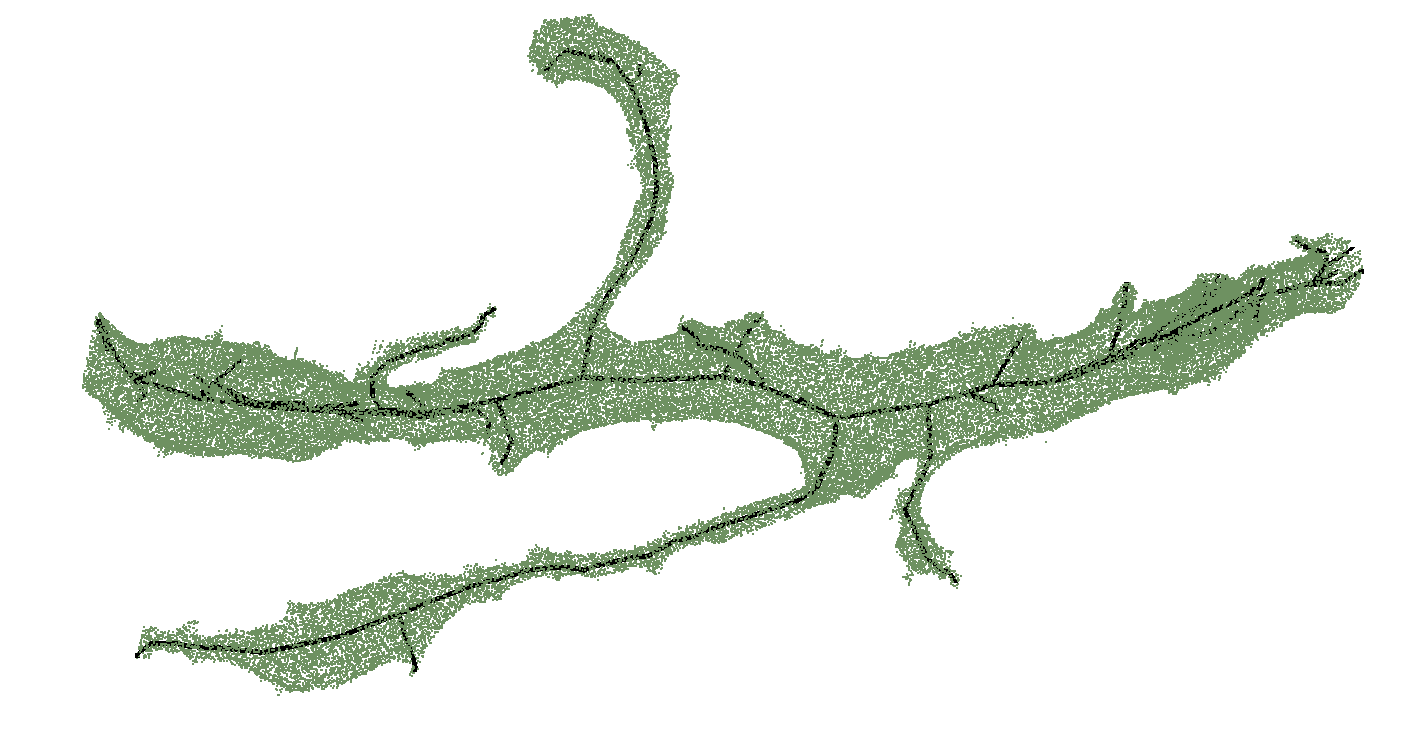
\includegraphics[width=\linewidth]{./figures/skeleton3.png}		
	\end{minipage}
	\hfill
	\begin{minipage}{0.45\linewidth}
		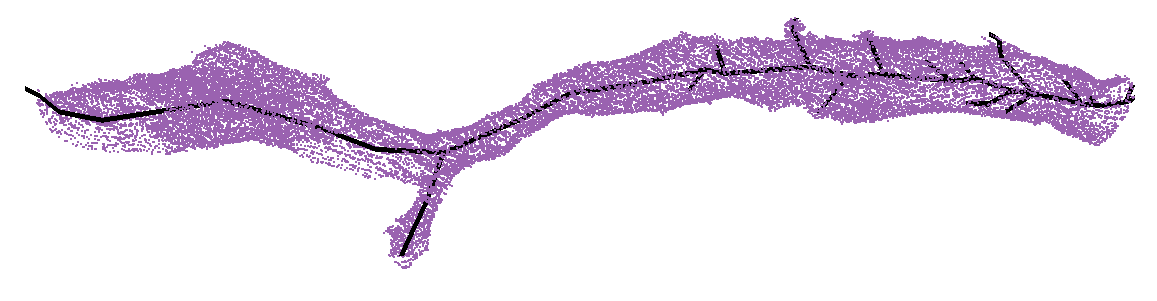
\includegraphics[width=\linewidth]{./figures/skeleton4.png}		
	\end{minipage}
	\caption{Example skeletons (in black) extracted from segments using a variant of the TEASER algorithm~\cite{sato2000teasar}. These skeletons not only capture the shape of the segmentation, but also provide endpoints useful for region merging proposals.}
	\label{fig:skeletonization}
\end{figure}

Our key observation is that if two segments belong to the same neuronal process, their skeleton end points should satisfy certain geometric constraints.
To extract the skeleton from each segment, we use a variant~\cite{zhao2014automatic} of the TEASER algorithm~\cite{sato2000teasar}. 
This skeletonization algorithm repeatedly uses Dijkstra's algorithm to find the farthest voxel from a seed location. 
Since this algorithm is non-linear in the number of voxels, we downsample the datasets so that there are voxel samples every $\SI{30}{\nano\meter}$ in each dimension.
Empirically, this reduced the running time for skeletonization by $30\times$ with minimal reduction in skeleton accuracy (${\sim}5\%$ fewer branches). 
Fig.~\ref{fig:skeletonization} shows four examples of extracted skeletons (in black). 
These skeletons consist of a sequence of \textit{joints}, locations that are locally a maximum distance from the segment boundary, with line segments connecting successive joints. 
We refer to joints that have only one connected neighbor as \textit{endpoints}. 
We find that approximately 70\% of the segments that are erroneously split have nearby endpoints (Fig.~\ref{fig:merge_candidates}). 

Two segments, $s_1$ and $s_2$, receive a corresponding edge if the two following conditions hold.
First, endpoints in either $s_1$ or $s_2$ are within $t_{low}$ nm of any voxel in the other segment.
Second, there are endpoints in $s_1$ and in $s_2$ that are within $t_{high}$ nm of each other.
We store the midpoints between the two endpoints as the center of the potential merge in the set $\mathbb{S}_c$. 
This algorithm produces a set of segments to consider for merging. 
Only these pairs have a corresponding edge in the constructed graph.
We provide an empirical analysis of these parameters on the structure of the graph in the supplemental materials.

\begin{figure}[t]
	\begin{minipage}{0.4\linewidth}
		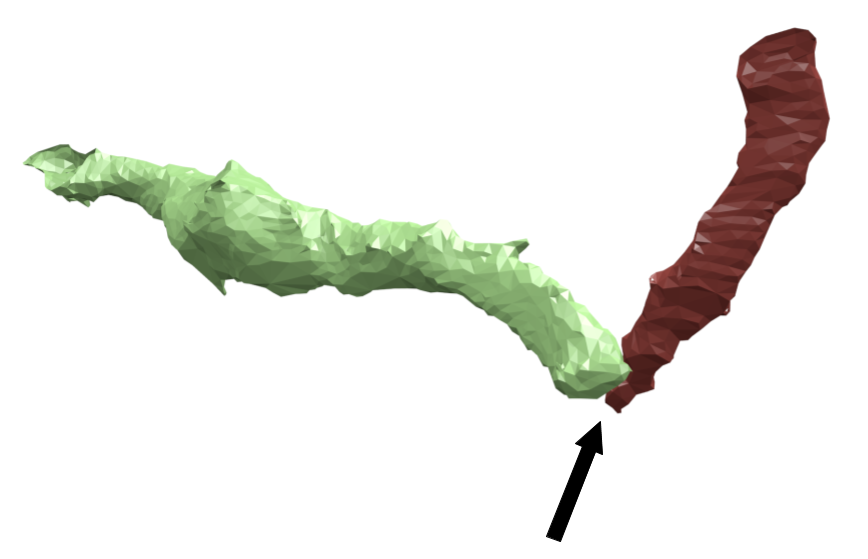
\includegraphics[width=\linewidth]{./figures/constraint_error.png}
	\end{minipage}
	\hfill
	\begin{minipage}{0.55\linewidth}
		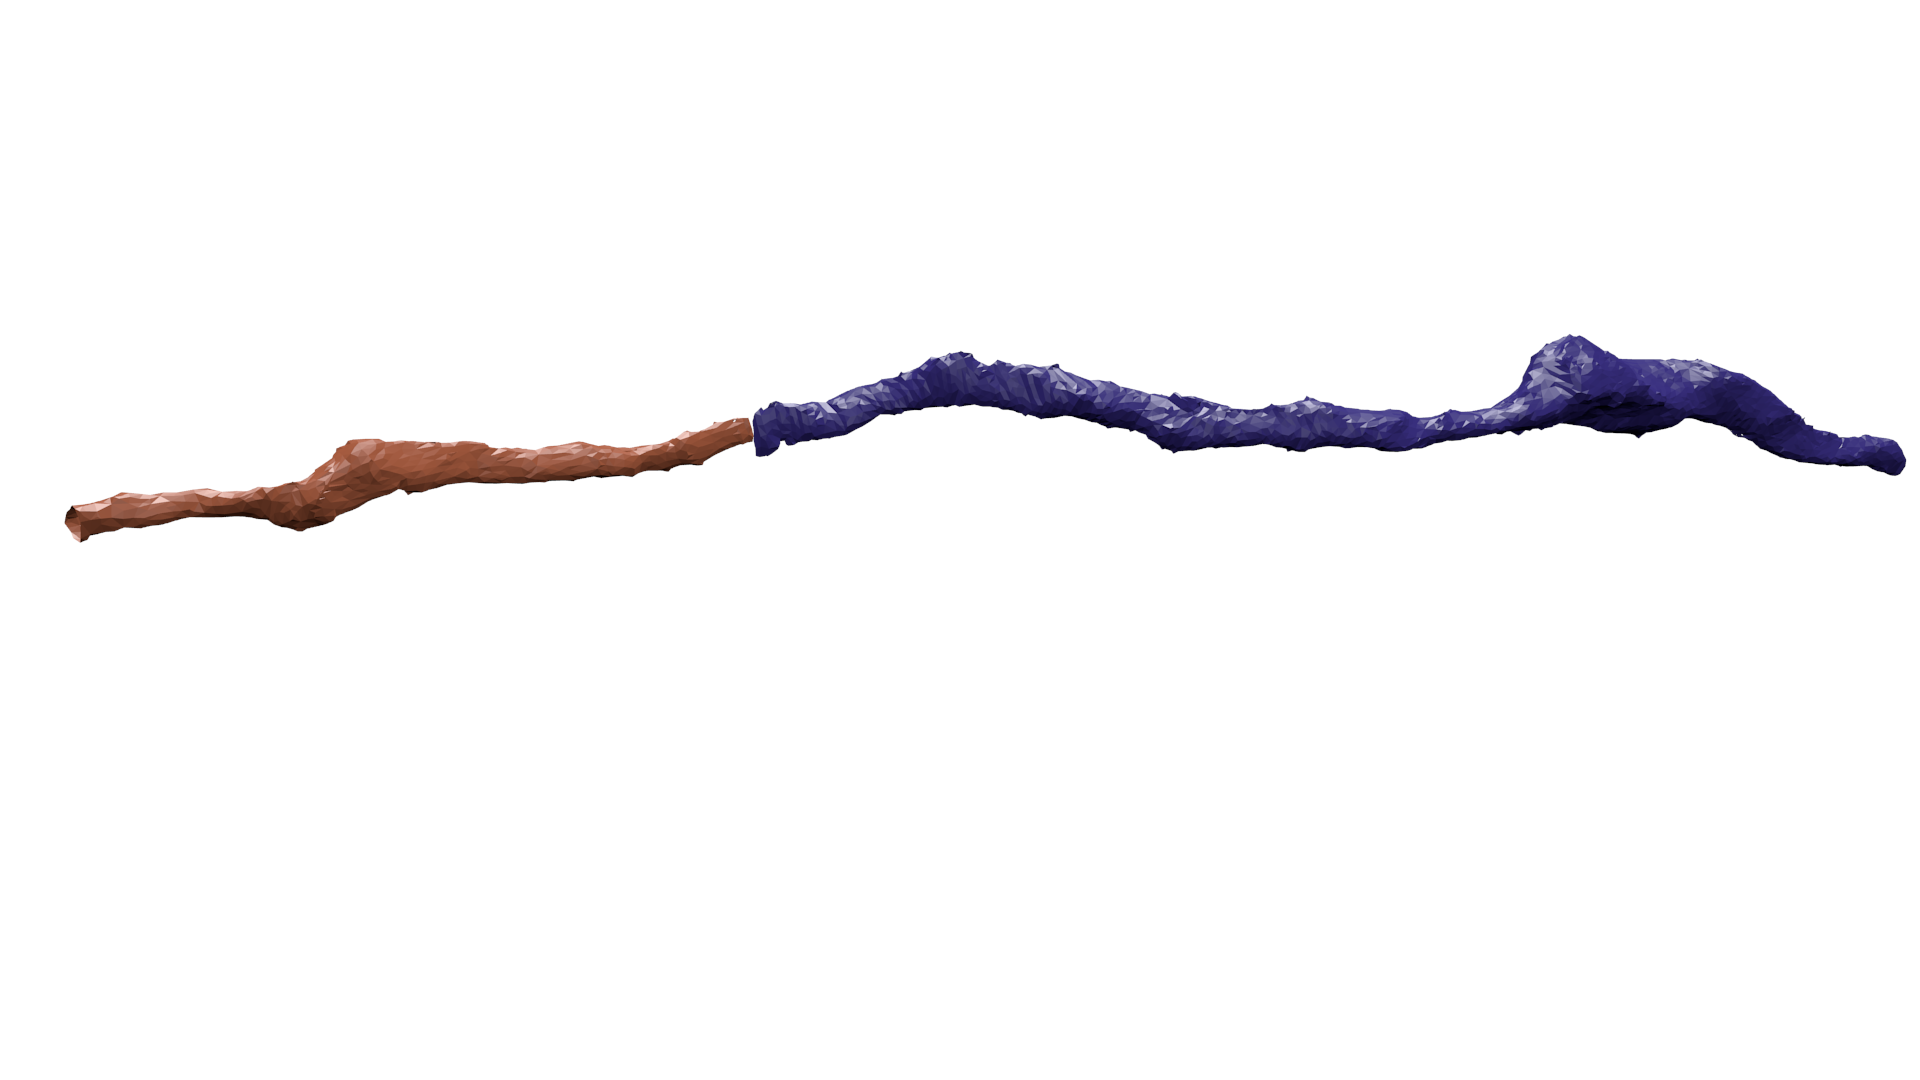
\includegraphics[width=\linewidth]{./figures/constraint_success.png}
	\end{minipage}
	\caption{Geometric constraints for region merging. We show two region merging proposals. On the left, the segments do not belong to the same neuron, as evidenced by the sharp turning radius indicated by the arrow; while on the right, the segments should be merged due to the continuity of the 3D shape. Instead of using handcrafted geometric features, we train a convolutional neural networks to automatically learn them from the ground truth labels.}
	\label{fig:turn-radii}
\end{figure}
\subsection{Learning-based Edge Weight}
\label{sec:edge-weights}
We assign an edge weight $w_e$ to each edge corresponding to the probability that two nodes belong to the same neuronal process.
We train a 3D CNN model to learn these geometric constraints for valid connection between two segments from labeled volume.
\\~\\
\noindent\textbf{Edge Probability}
To predict the probabilities that two segments belong to the same neuron, we train a feed-forward convolutional network with three \textit{VGG-style} convolution blocks~\cite{chatfield2014return} and two fully connected layers before the final sigmoid activation. 

For the input of the network, we extract a cubic region of interest (ROI) around each endpoint $e$ in $\mathbb{S}_c$ as input to the CNN. 
The CNN receives three input channels for every voxel in the ROI around segments $l_1$ and $l_2$. 
The input in all of the channels is in the set $\{-0.5, 0.5\}$. 
The first channel is $0.5$ only if the corresponding voxel has label $l_1$. 
The second channel is $0.5$ only if the corresponding voxel has label $l_2$. 
The third channel is $0.5$ if the corresponding voxel is either $l_1$ or $l_2$.
We do not use the raw EM image information to avoid the need to retrain the network on datasets that have been stained differently or imaged at different resolution. 
This reduces the need for generating costly manually-labeled ground truth. 

\begin{figure}[t]
	\centering
	\begin{minipage}{0.32\linewidth}
		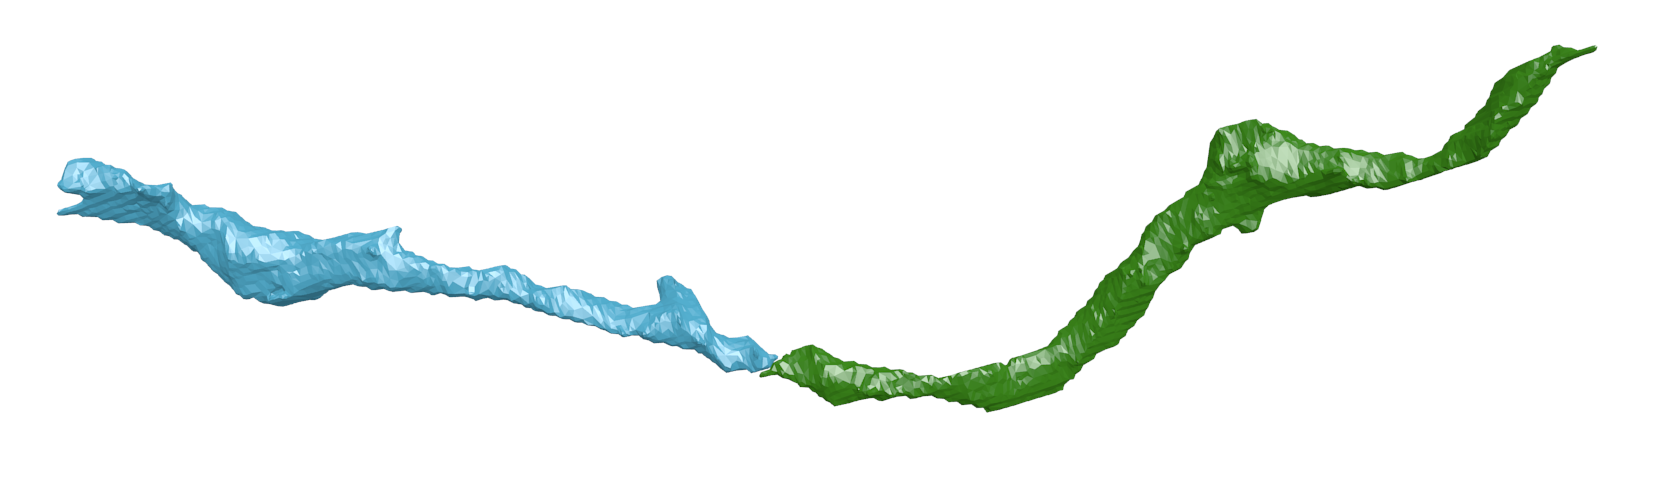
\includegraphics[width=\linewidth]{./figures/split_error1.png}		
	\end{minipage}
	\hfill
	\begin{minipage}{0.32\linewidth}
		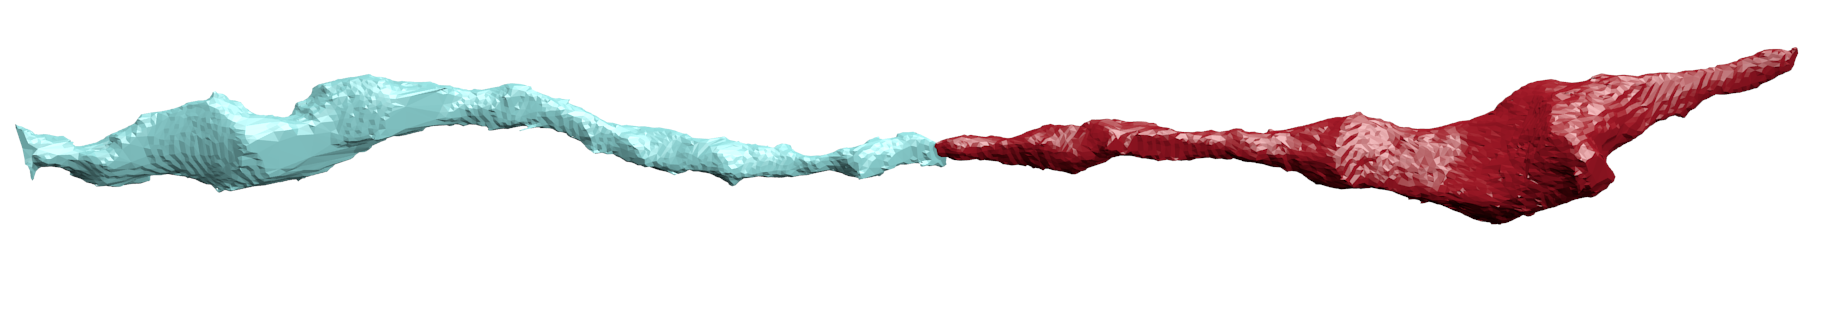
\includegraphics[width=\linewidth]{./figures/split_error2.png}				
	\end{minipage}
	\hfill
	\begin{minipage}{0.32\linewidth}
		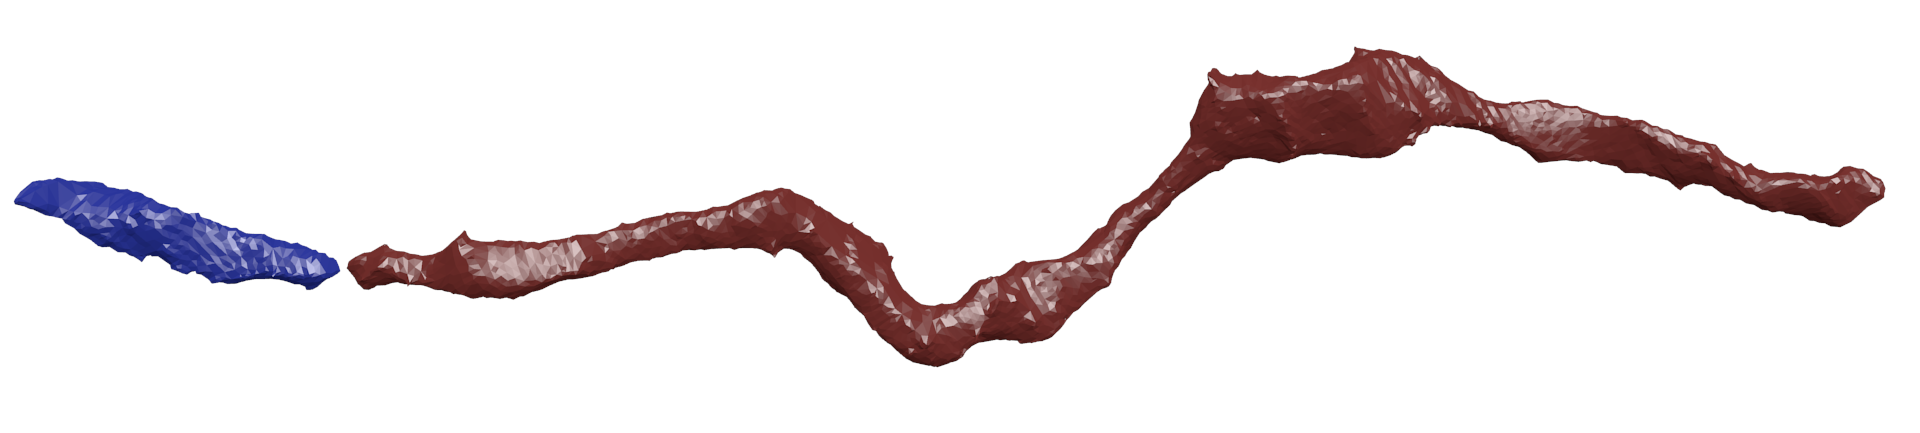
\includegraphics[width=\linewidth]{./figures/split_error3.png}
	\end{minipage}
	\caption{Three erroneously split segments.}
	\label{fig:merge_candidates}
\end{figure}
\subsection{Optimization-Based Graph Partition}
\label{sec:optimization}
After graph construction, we segment the graph in a globally consistent manner while enforcing topological constraints on the output.
\\~\\
%\subsubsection{Lifted Multicut}
\noindent\textbf{Lifted Multicut}
After constructing the graph we seek to partition it into labels where every label corresponds to a neuronal process. 
We formulate this graph partitioning problem as a multicut problem.
There are two primary benefits to using a multicut formulation. 
First, the number of segments in the final graph is not predetermined but depends on the input. 
Second, this minimization produces globally consistent solutions (i.e., a boundary remains only if the two corresponding nodes belong to unique segments)~\cite{keuper2015efficient}.

We apply the algorithms of Keuper et al.~\cite{keuper2015efficient} to produce a feasible solution to the multicut problem using greedy additive edge contraction.
Following their example, we employ the generalized lifted multicut formulation.
Traditional multicut solutions only consider the probabilities that two adjacent nodes belong to the same segment. 
In the lifted extension to the problem, we can penalize non-adjacent nodes that belong to different segments. 
These penalties between non-adjacent nodes are called lifted edges. 
Ideally these lifted weights represent the probability that two nodes belong to the same neuron.
However, determining such probabilities is computationally expensive.
We approximate these probabilities by finding the maximal probable path between any two nodes using Dijkstra's algorithm~\cite{keuper2015efficient}.
This is an underestimate of the probability that two nodes belong to the same neuron since it does not consider all possible paths.
Since our graphs are sufficiently small, we can generate lifted edges between all pairs of nodes. 
\\~\\
\noindent\textbf{Edge Weight} 
We need to convert the probabilities into the following weighting scheme to solve the multicut problem with this heuristic~\cite{keuper2015efficient,andres2011probabilistic}.
Given the probability that the nodes belong to the same neuron is $p_e$, the edge weight $w_e$ is defined as
%p_e &=\mbox{CNN}(x_1, x_2) \\
\begin{align}
w_e = \log{\frac{p_e}{1 - p_e}} + \log{\frac{1 - \beta}{\beta}},
\end{align}
where $\beta$ is a tunable parameter that encourages over- or under-segmentation. 
Since, there are many more lifted edges than adjacent edges, we scale down the lifted weights proportionally to their total number  
~\cite{beier2017multicut}.
\\~\\
%\subsubsection{Topological Constraints}
\noindent\textbf{Topological Constraints}
By reformulating the segmentation problem as a graph partitioning one, we can enforce some global constraints on our result based on the underlying biology.
Traditional hierarchical clustering algorithms do not rely on such constraints but consider local decisions independently.
We enforce a global constraint that neurons are tree-structured and should not contain cycles. 
The multicut problems returns a series of ``collapsed'' edges between nodes that belong to the same neuron.
We iterate over these edges in order of the probability of merge generated by our CNN. 
We ``collapse'' an edge only if it does not create a cycle in the graph.

\paragraph{Compression}

\begin{figure*}[t]
	\begin{center}
		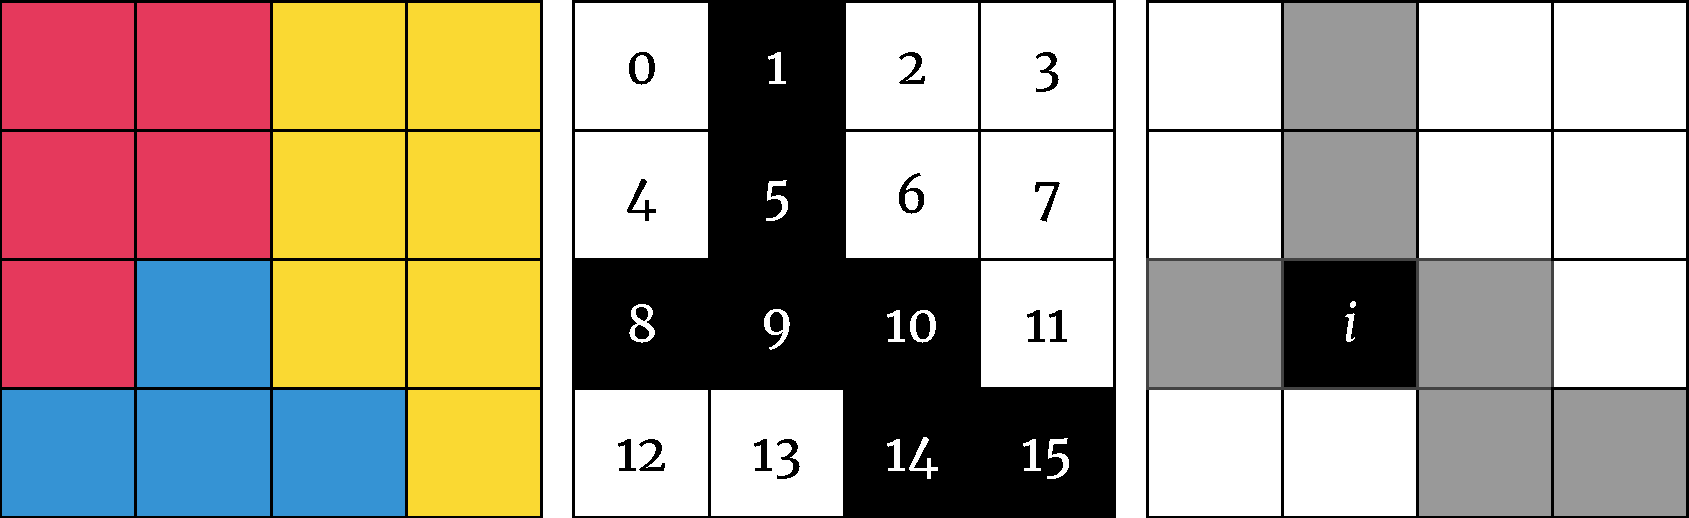
\includegraphics[width=0.45\linewidth]{./figures/encoding_diagram_opt.pdf}
		\hspace{0.08\linewidth}
		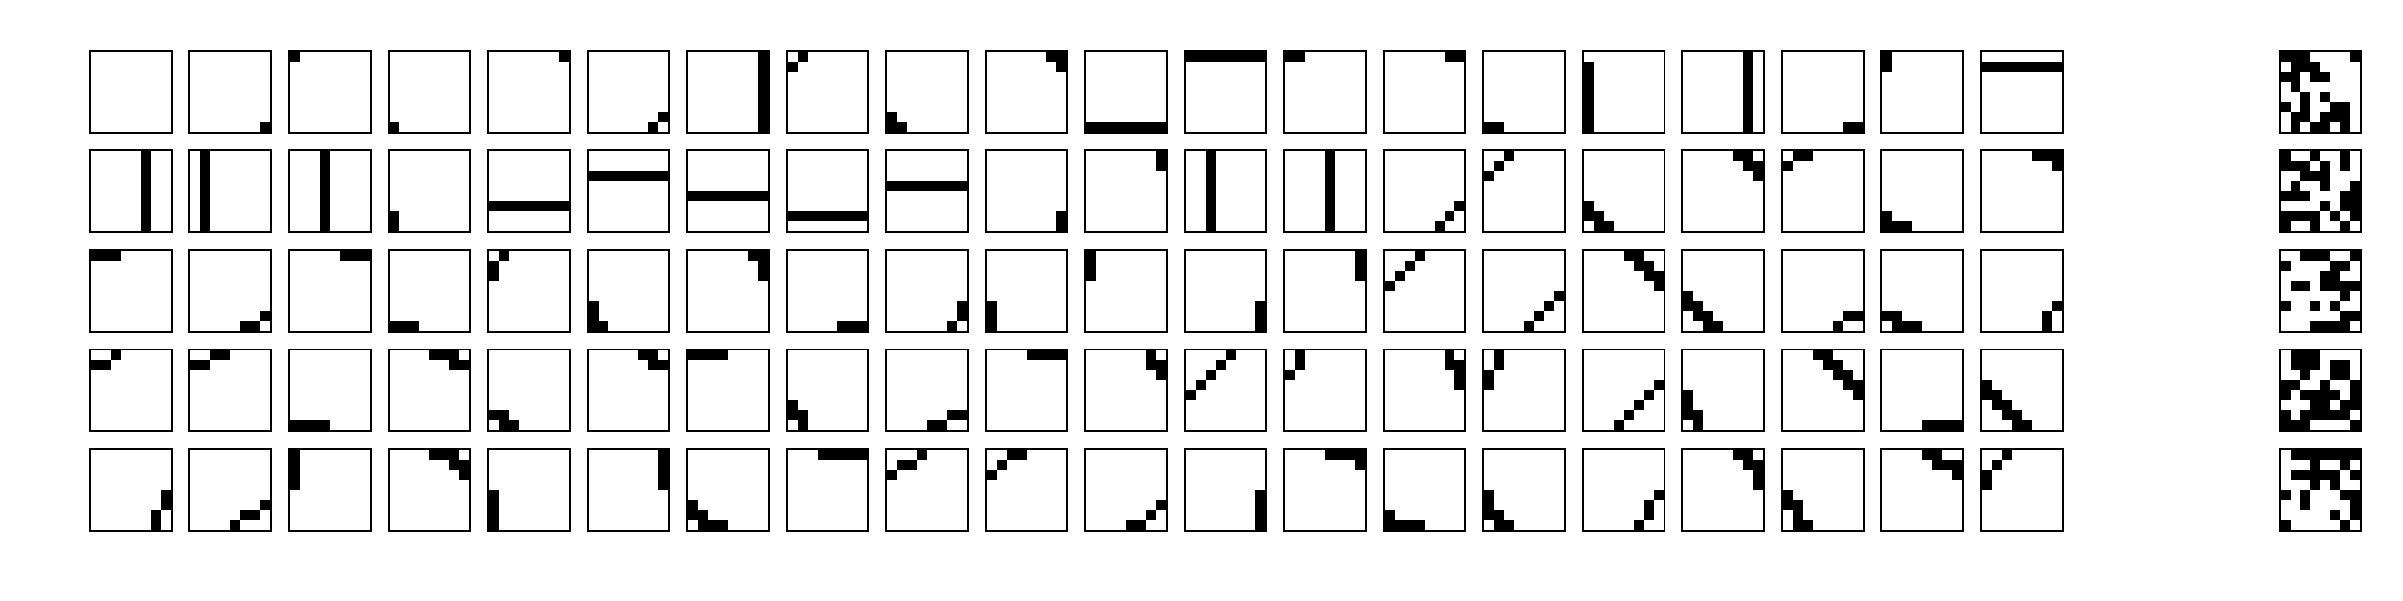
\includegraphics[width=0.45\linewidth]{./figures/window_values.pdf}
	\end{center}	
	\caption{Compresso works by dividing up the segmentation data into small blocks. On the left we show the intersection of three segments in a $4\times4\times1$ window. We extract a boundary map from this segmentation to transform the window into an integral value between $0$ and $2^{16} - 1$. The location $i$ requires some additional bookkeeping. On the right are the $100$ most common $8 \times 8 \times 1$ windows accounting for $\sim82\%$ of the volume on a representative dataset.}
	\label{fig:compression}
\end{figure*}

Segmentation datasets contain two important pieces of information across the image stack: per-segment shape and per-pixel label. 
Decoupling these two components allows for better compression on each.

\paragraph{Boundary Encoding.}
\label{sec:boundary-map}

To encode the segment shapes, we consider the boundary pixels between two segments. 
Removing the per-pixel labels, we produce a boundary map for each slice where a pixel $(x, y, z)$ is 1 if either pixel at $(x + 1, y, z)$ or $(x, y + 1, z)$ belongs to a different segment. 
The boundary map is divided into non-overlapping congruent 3D windows. If there are $n$ pixels per window, each window $w$ is assigned an integer $V_w \in [0, 2^n)$ where $V_w$ is defined as:

\begin{equation}
V_w = \sum_{i = 0}^{n - 1} \mathbb{I}(i) 2^i,
\end{equation}

\noindent
and $\mathbb{I}(i)$ is 1 if pixel $i$ is on a boundary and 0 otherwise. 
Figure~\ref{fig:bockwurst-encoding} shows an example segmentation with a window size of $4 \times 4 \times 1$.


A priori, each window could take any of $2^n$ distinct values, and therefore require $n$ bits to encode without further manipulation. 
However, boundaries in segmentation images are not random, and many of these values never appear. 
Indeed, we find that a small subset of high-frequency $V_w$ values accounts for most windows, allowing for significant compression. 
Figure~\ref{fig:bockwurst-frequency} shows the 100 most common windows for a representative connectomics dataset. 
These 100 frequently occurring windows account for approximately 82\% of the over 1.2 million $V_w$ values in this dataset.
Nearly all of these windows correspond to simple lines traversing through the window. 
For contrast, we also provide 5 randomly generated windows that never occur in the dataset.

We define $N$ as the number of distinct $V_w$ representing all of the windows in an image stack. 
We construct an invertible function $f(V_w) \to [0, N)$ to transform the window values into a smaller set of integers. 
For all real-world segmentations $N \ll 2^n$; however, we assume no constraint on $N$ in order to guarantee lossless compression. 
With this function, each $V_w$ requires $\log_2{N}$ bits of information to encode. 
This is fewer than the initial number of bits so long as $N \leq 2^{n - 1}$.  
We create two arrays that store the per-segment shape encoding: $\texttt{WindowValues[]}$ contains the value $f(V_w)$ for every window $w$ and $\texttt{ValueMapping[]}$ contains the reverse mapping from $[0, N) \to [0, 2^n)$ based on the function $f$. 
Long sequences of $0$s in $\texttt{WindowValues[]}$ are reduced using run-length encoding.

\paragraph{Per-Pixel Label Compression.}

So far we have focused exclusively on transforming the boundary map of an image segmentation. 
However, the per-pixel labels themselves are equally important. 
The boundary map divides each image slice into different segments. 
By design, all pixels in the same segment have the same label so we store only one label per segment for each slice. 
We use a connected-component labeling algorithm to store one label per segment \cite{he2009fast}. 
The algorithm labels all pixels clustered within a component $m$ from $M$ section labels.
We store the original label for a segment $m$ in slice $z$ in $\texttt{Labels}_z\texttt{[m]}$. 
We concatenate these arrays for every image slice to create a variable $\texttt{Labels[]}$.

\paragraph{Exceptions.}

Thus far, we have assumed the boundaries described in Section~\ref{sec:boundary-map} provide enough information to reconstruct the entire segmentation.
Pixels not on a segment boundary are easily relabeled using the $\texttt{Labels[]}$ array. 
However, more care is needed for pixels on the segment boundaries. 
Consider Figure~\ref{fig:bockwurst-encoding}, which depicts a difficult boundary to decode. 
If a boundary pixel has a non-boundary neighbor to the left or above, then that pixel merely takes on the value of that neighbor. 
However, the pixel $i$ requires more care since its relevant neighbors are both boundary pixels. 
If a non-boundary neighbor pixel shares a label with the undetermined pixel, we add the offset to that neighbor to an array \texttt{IndeterminateValues[]}. 
Otherwise we add that per-pixel label.

\paragraph{Metadata.}

We construct a data structure containing the two per-segment shape and two per-pixel label arrays. The last component of the data structure is the \texttt{Header}, which contains the dimensions of the original data, the window size, and the size of the arrays. Compresso could be improved by further compressing the individual components of the encoding (e.g., Huffman encoding the $V_w$ values). We achieve strong overall compression by using a second-stage general compression scheme such as LZMA~(Sec.~\ref{sec:results}).


\subsection{Decoding}

The first step in decoding the data is to reconstruct the boundary map. We iterate over every pixel, determine the corresponding window $w$, and retrieve the encoded window value $f(V_w)$ from the $\texttt{WindowValues[]}$ array. These values range from $0$ to $N - 1$ and correspond to an index in $\texttt{ValueMapping[]}$ that contains the original $V_w$ value. After decoding $V_w$, the value of pixel $i$ in window $w$ equals $V_w \land 2^i$.

After reproducing the boundary map, we execute the same deterministic connected-components algorithm per slice as when encoding. Each component in the boundary map receives a label between $0$ and $M - 1$. Using the $\texttt{Labels[]}$ array, we can easily translate these component labels into the original per-pixel labels for every slice. To determine the per-pixel labels for every boundary pixel, we iterate over the entire dataset in raster order. Any boundary pixel $(x, y, z)$ with a non-boundary neighbor at $(x - 1, y, z)$ or $(x, y - 1, z)$ shares the same per-pixel label. If both relevant neighbors are boundaries we consider the next unused value in the $\texttt{IndeterminateValues[]}$ array and update this pixel's label.


